\begin{titlepage}
\centering
\noindent\rule{\textwidth}{1pt} \par

\vspace{1cm}
\noindent
\begin{minipage}[c]{0.25\textwidth}
    \flushleft
\includegraphics[width=\textwidth, height=2.5cm, keepaspectratio]{Images/logocomp.png}
\end{minipage}
\hfill
\begin{minipage}[c]{0.45\textwidth}
    \centering
    \LARGE\textbf{MASTER'S THESIS}\\[5mm]
    \footnotesize mention Physique fondamentale \& applications, spécialité Physics \& Computational Physics
\end{minipage}
\hfill
\begin{minipage}[c]{0.25\textwidth}
    \flushright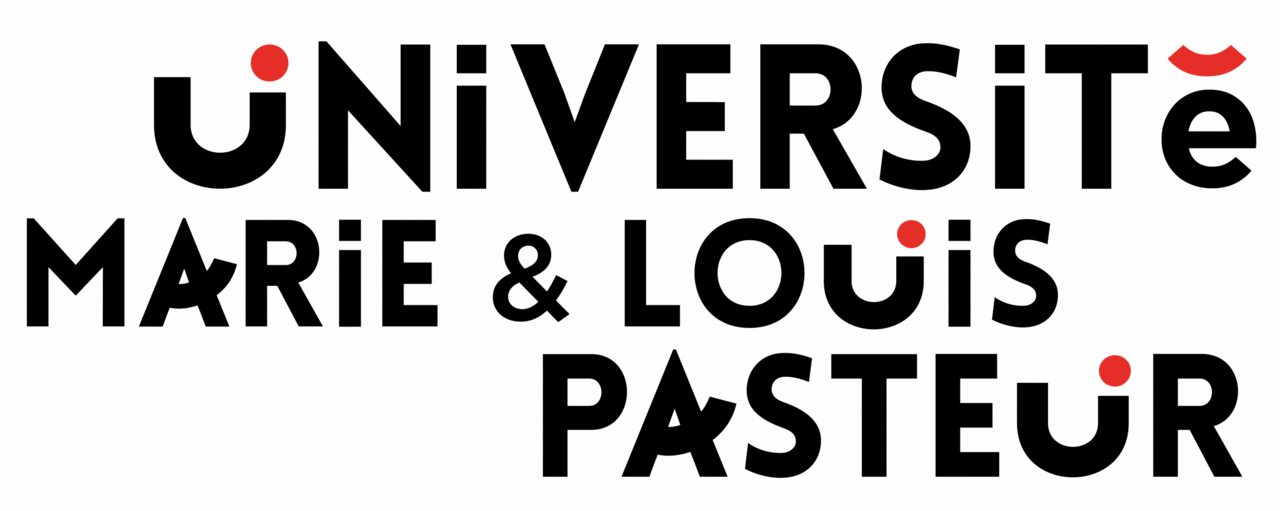
\includegraphics[width=\textwidth, height=2.5cm, keepaspectratio]{Images/logo.png}
\end{minipage}

\vspace{0.8cm}
\rule{0.7\textwidth}{1pt} \par

\vspace{5cm}\Huge
\textbf{Evolution of open quantum systems}\\[0pt]
\textbf{under continuous measurement}\\[0pt]
\textbf{of their environment}
\vspace{2cm}

\normalsize
% STUDENT + SUPERVISOR*
\vfill
\noindent
\begin{minipage}[t]{0.48\textwidth}
    \raggedright% Aligné à gauche
    \textbf{STUDENT:} \\
    Jules STEVENOT
\end{minipage}
\hfill
\begin{minipage}[t]{0.48\textwidth}
    \raggedleft% Aligné à droite
    \textbf{SUPERVISOR:} \\
    Bruno BELLOMO\footnotemark[1]
\end{minipage} \par

% LOGO + DATE
\begin{minipage}[c]{0.25\textwidth}
    \flushleft
\includegraphics[width=\textwidth, height=2.5cm, keepaspectratio]{Images/logoPTH.png}
\end{minipage}
\hfill
% \begin{minipage}[c]{0.45\textwidth}
%     \centering {\textit{January-June 2026}}
% \end{minipage}
% \hfill
\begin{minipage}[c]{0.25\textwidth}
    \flushright
\includegraphics[width=\textwidth, height=2.5cm, keepaspectratio]{Images/logoUTI.jpeg}
\end{minipage}
\footnotetext[1]{Equipe $\Phi$Th, Institut UTINAM - CNRS 6213, OSU THETA.}\par
January-June 2026\\[5mm]
\end{titlepage}
\clearpage\thispagestyle{empty}\null%